\section{Evaluation}
\label{eval}

\subsection{YFCC100M Dataset}
\label{dataset}

\textbf{\textit{Here goes an explanation of the dataset and all the source
(images, metadata, videos, features).}}

We use the Yahoo! Flickr Creative Commons 100m (YFCC100M) dataset ~\cite{Thomee_2016} for a large collection of 100 million public Flickr media objects.  This dataset contains approximately 99.2 million images and 0.8 million videos along with respective metadata characterized by 25 fields such as the identifier (metaid), the user who created the media (image/video), the date the media was taken and uploaded, the longitude/latitude it was taken, and the device the media was captured from.  The metadata also provides information including the URL to download the media, a title, a description of the media, user and machine tags, and license information.  To understand the content of the media, the YFCC100M also provides autotags which is a set of comma-separated tags and confidence scores generated from 1,570 trained Caffe binary SVM classifiers.  

\subsection{Experimental Setup}

\textbf{\textit{Here goes explanation of the comparison systems.
Need versions of MySQL, OS, amount of memory and CPU info.}}

\begin{figure*}[]
\centering
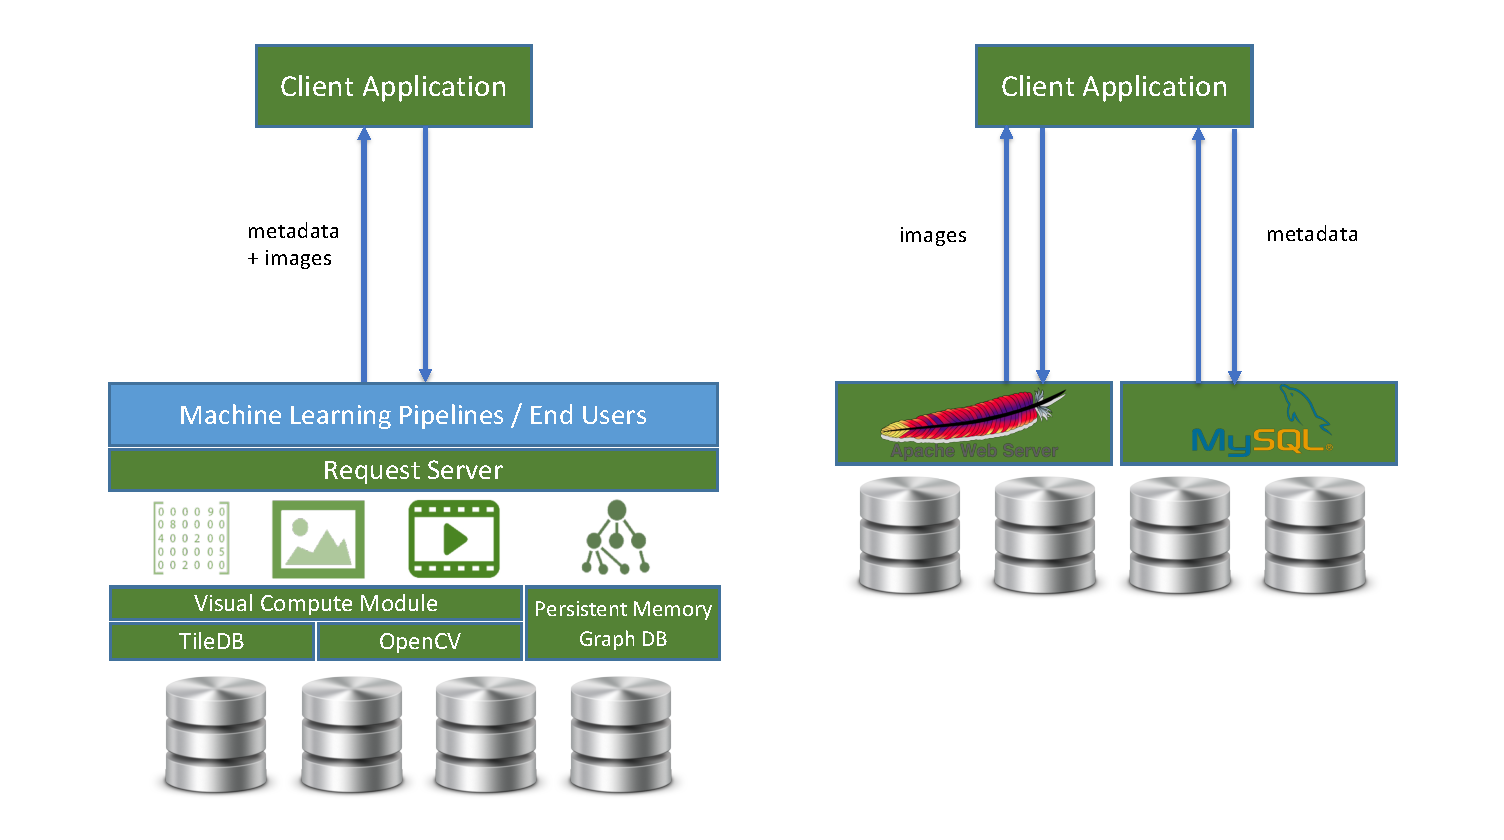
\includegraphics[width=\textwidth]{figures/comparison_system}
\caption{Comparison Systems}
\label{fig:systems}
\end{figure*}

As a baseline, we implemented a similar database system, depicted in Figure~\ref{fig:systems}, with popular components: MySQL Server 5.7, Apache Web Server, and OpenCV.  Each database system used the following configuration: Intel\textsuperscript{\textregistered} Xeon\textsuperscript{\textregistered} Platinum 8180 CPU @ 2.50GHz (Skylake) server running Ubuntu 16.04.  
 
For the experiments, we built VDMS and MySQL databases for the YFCC100M dataset for dataset sizes 100k, 500k, 1M, 5M, 10M, 50M, and 100M. The VDMS Python client library was used to build queries to insert the necessary elements to build the database.  In the database, we insert the edges for the 1570 autotags and the YFCC media objects with the appropriate metadata. To add the autotag confidence scores, we parse the autotag data and add a connection between the media object and tag edges with metadata denoting its appropriate confidence score. Table~\ref{table:vdmsedges} shows the number of elements in each database.  

\begin{table}[h]
\caption{Edges in VDMS database}
\centering
\begin{tabular}{c c c c}
\hline\hline
Database Size & No. Connections & Metadata (Images) & Autotags\\
\hline
100k & 848,432 & 100,000 & 1,570\\
500k & 4,249,500 & 500,000 & 1,570\\
1M & 8,503,045 & 1,000,000 & 1,570\\
5M & 42,505,478 & 5,000,000 & 1,570\\
10M & 85,040,404 & 10,000,000 & 1,570\\
50M & 425,162,070 & 50,000,000 & 1,570\\
100M & 895,572,430 & 99,205,984 & 1,570\\
\hline
\end{tabular}
\label{table:vdmsedges}
\end{table}

Alternatively, three tables were created for the MySQL system: taglist, metadata, and autotags.  The number of rows in the MySQL databases are shown in Table~\ref{table:mysqltables}. The taglist table contains the 1570 YFCC100M autotags where each entry is given an integer key named tagid.  The metadata table contains image metadata where the metadata identifier is the primary key. The autotags table contains the confidence scores for the generated autotags for metadata entries of the metadata table, the tagid associated with the autotag, and the metaid associated with the metadata identifier. 


\begin{table}[h]
\caption{Rows in MySQL database}
\centering
\begin{tabular}{c c c c}
\hline\hline
 & \multicolumn{3}{c}{Table}\\
\cline{2-4}
Database Size & Autotags & MetaData & Tag List\\
\hline
100k & 848,912 & 100,000 & 1,570\\
500k & 4,241,200 & 498,707 & 1,570\\
1M & 8,508,380 & 1,000,000 & 1,570\\
5M & 42,425,905 & 4,987,379 & 1,570\\
10M & 85,095,265 & 10,000,000 & 1,570\\
50M & 425,446,208 & 50,000,000 & 1,570\\
100M & 896,002,496 & 99,206,564 & 1,570\\
\hline
\end{tabular}
\label{table:mysqltables}
\end{table}

The VDMS and MySQL databases have comparable number of elements as shown in Table~\ref{table:vdmsedges} and ~\ref{table:mysqltables} but on average it takes MySQL 3.7x hours longer to build than VDMS. Figure~\ref{fig:db_time_size} compares the time to build and the size of the VDMS and MySQL databases. VDMS requires approximately 1.4x more storage than MySQL each database.  This is due to the need to store relationship information for the graph database.

\begin{figure}[]
\centering
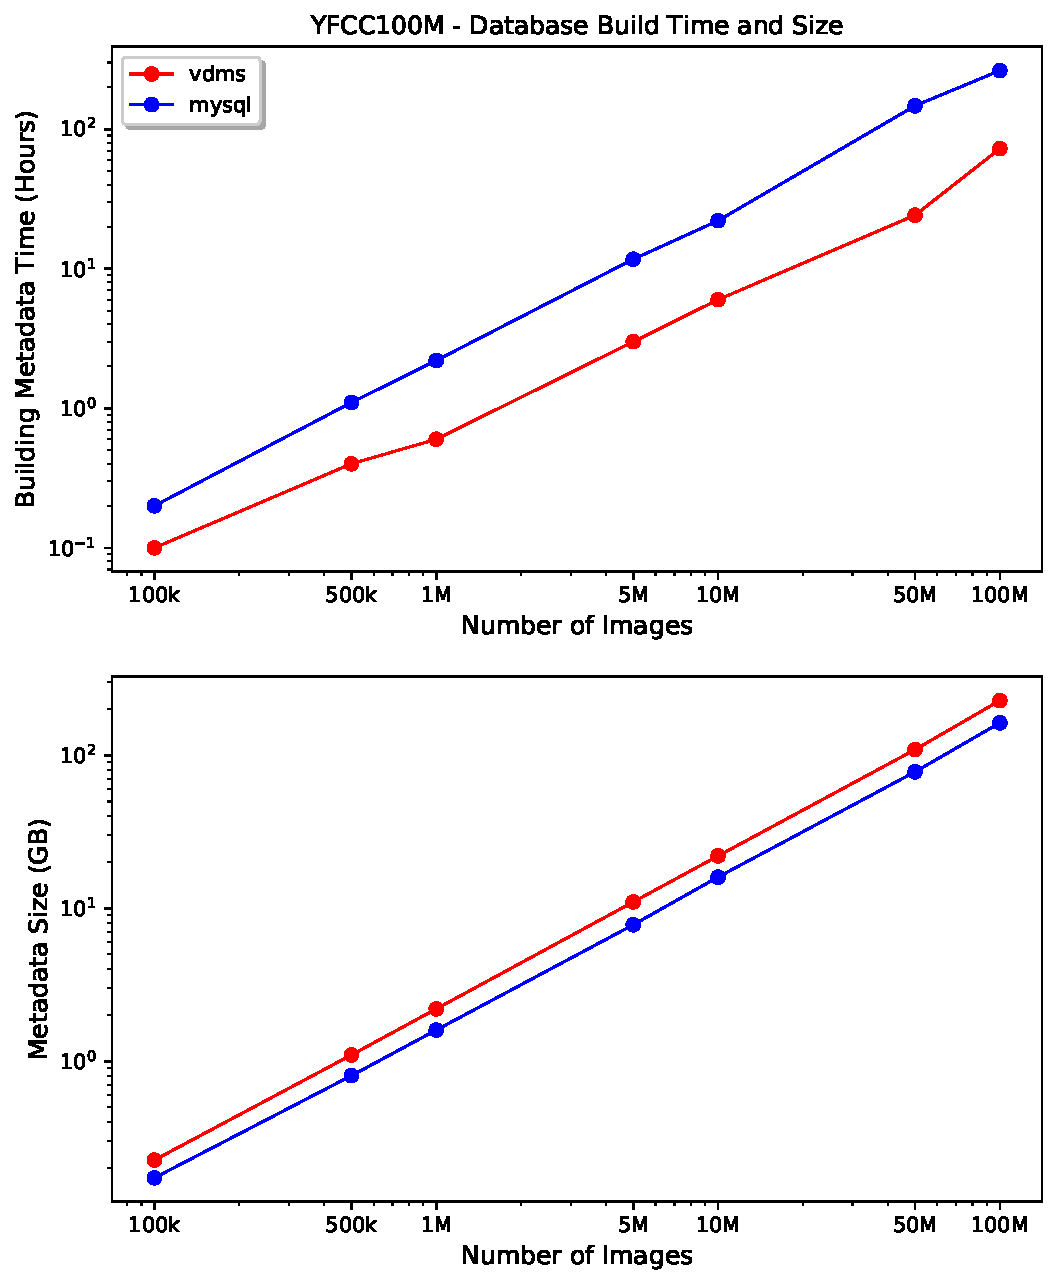
\includegraphics[width=\columnwidth]{figures/db_time_size}
\caption{Time (in hours) to build and size (in GB) of MySQL and VDMS databases}
\label{fig:db_time_size}
\end{figure}


\subsection{Images + Metadata}

\textbf{\textit{Explanation of the evaluation and description of some of the queries.}}

\begin{figure}[]
\centering
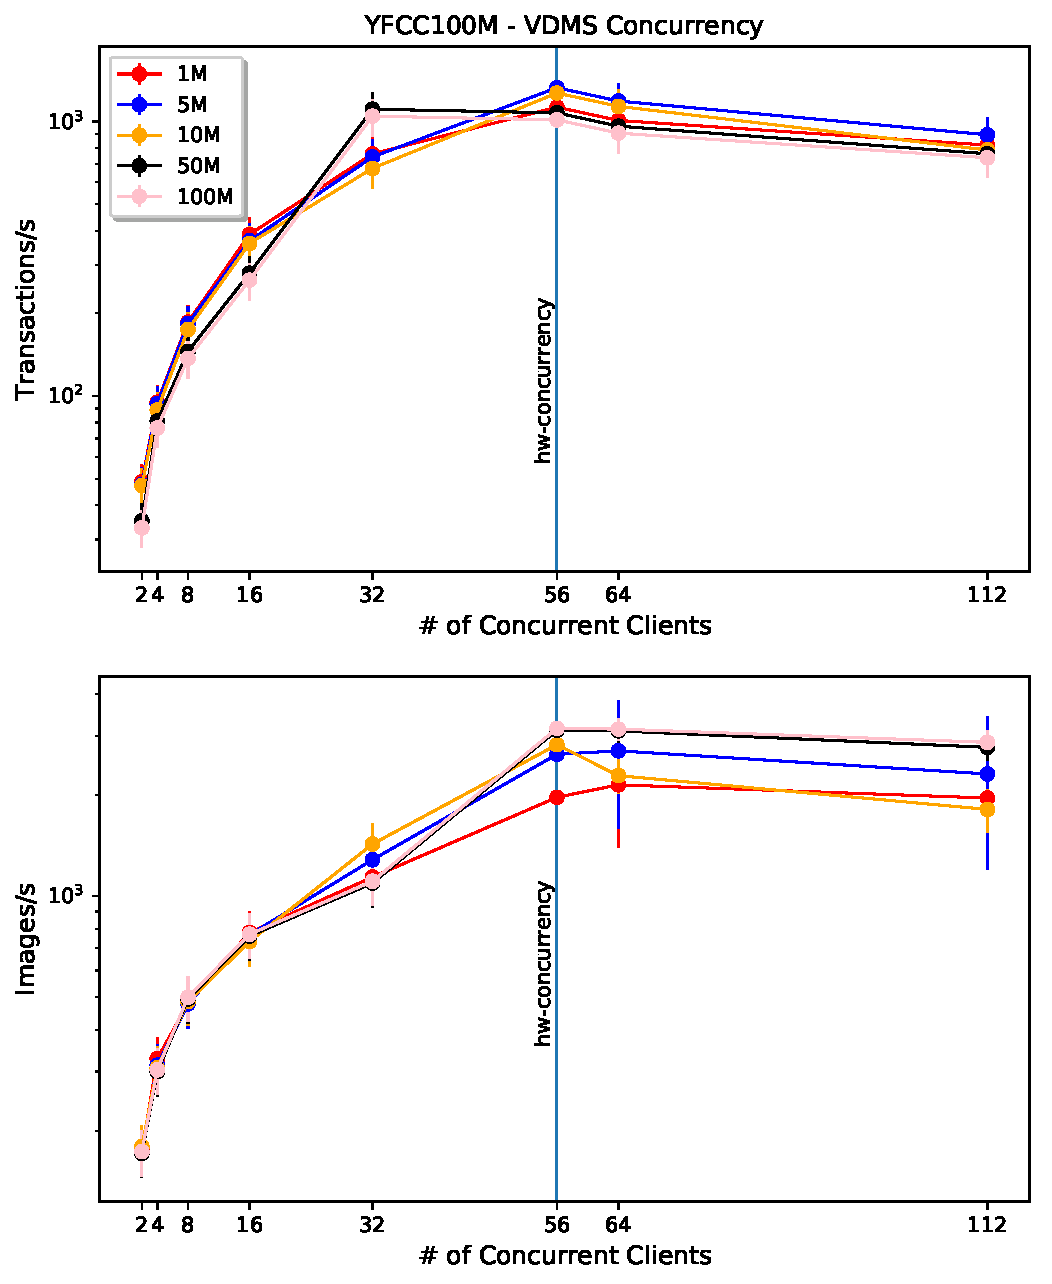
\includegraphics[width=\columnwidth]{figures/concurrency_vdms}
\caption{Concurrency Analisys - VDMS}
\label{fig:concurrency_vdms}
\end{figure}

\begin{figure}[]
\centering
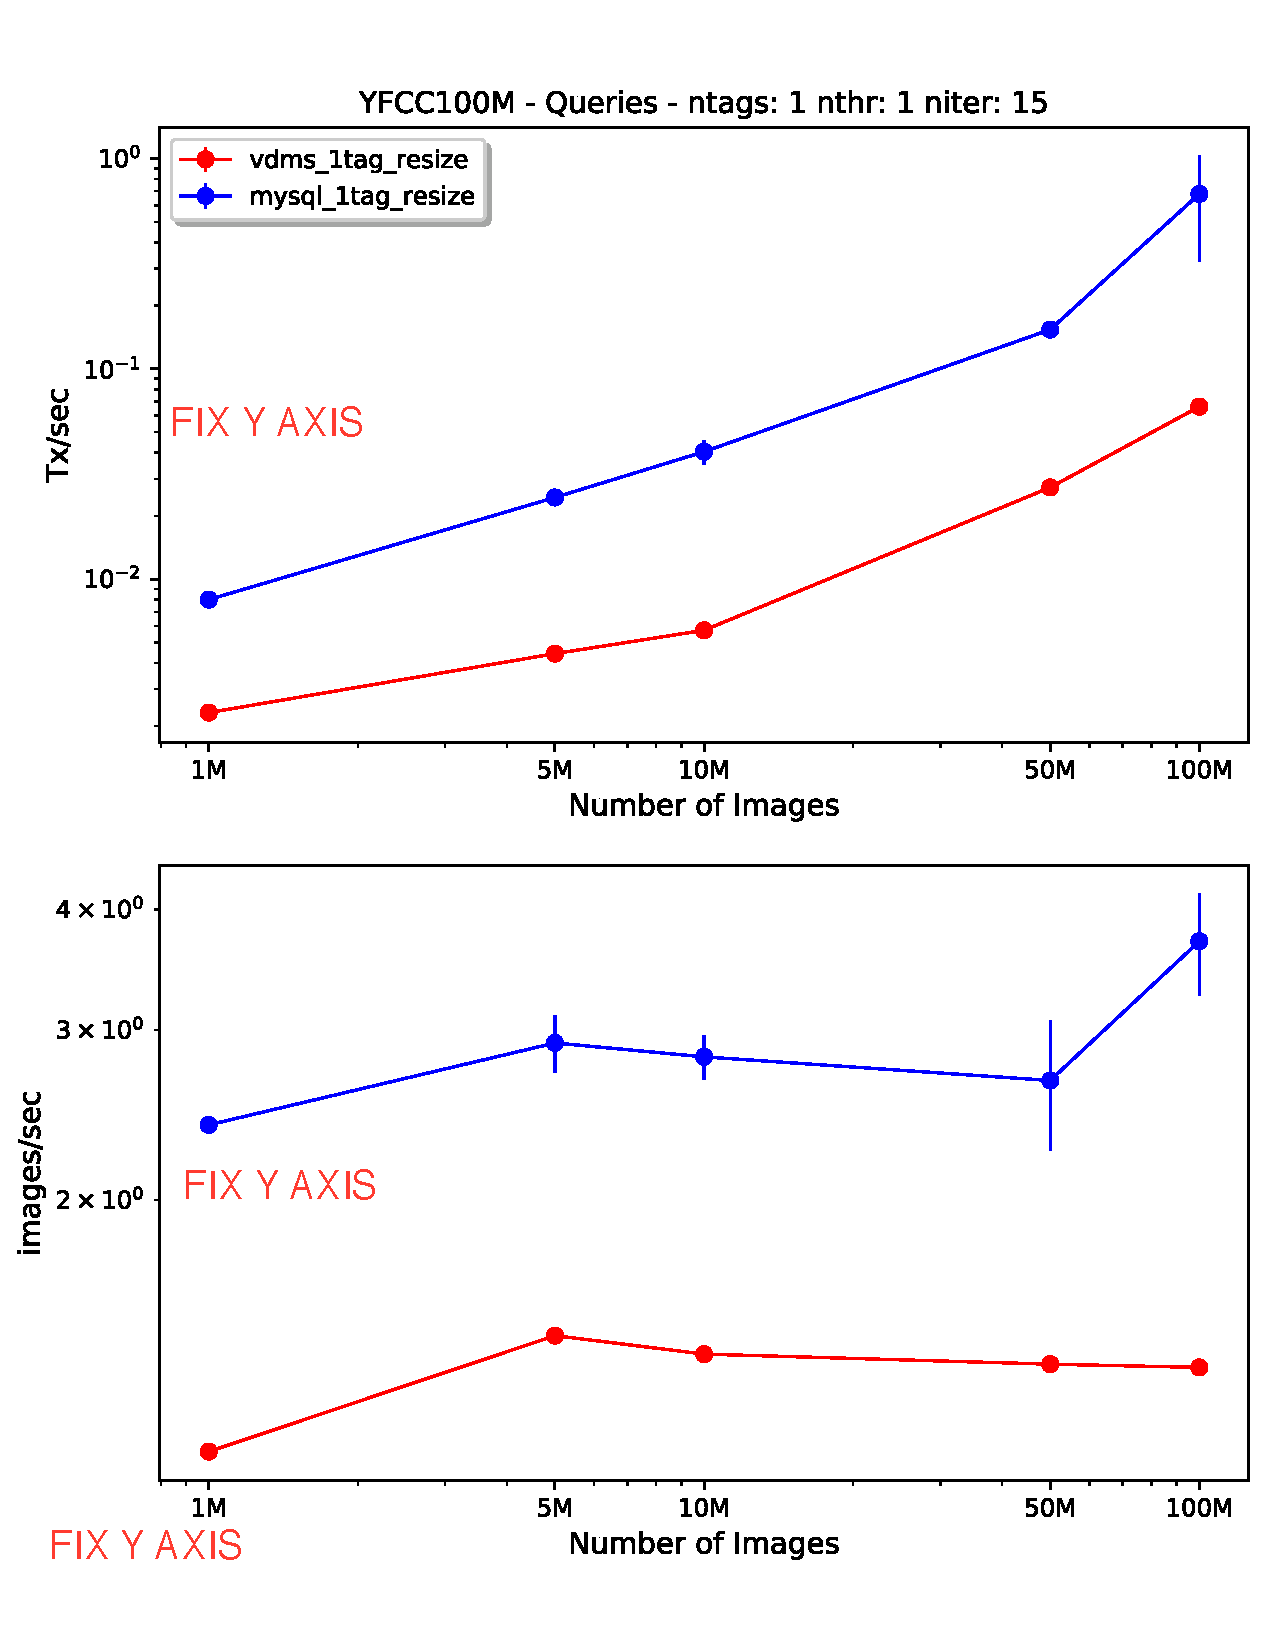
\includegraphics[width=\columnwidth]{figures/q1_latency}
\caption{Query 1 - Latency}
\label{fig:q1_latency}
\end{figure}

\begin{figure}[t!]
\centering
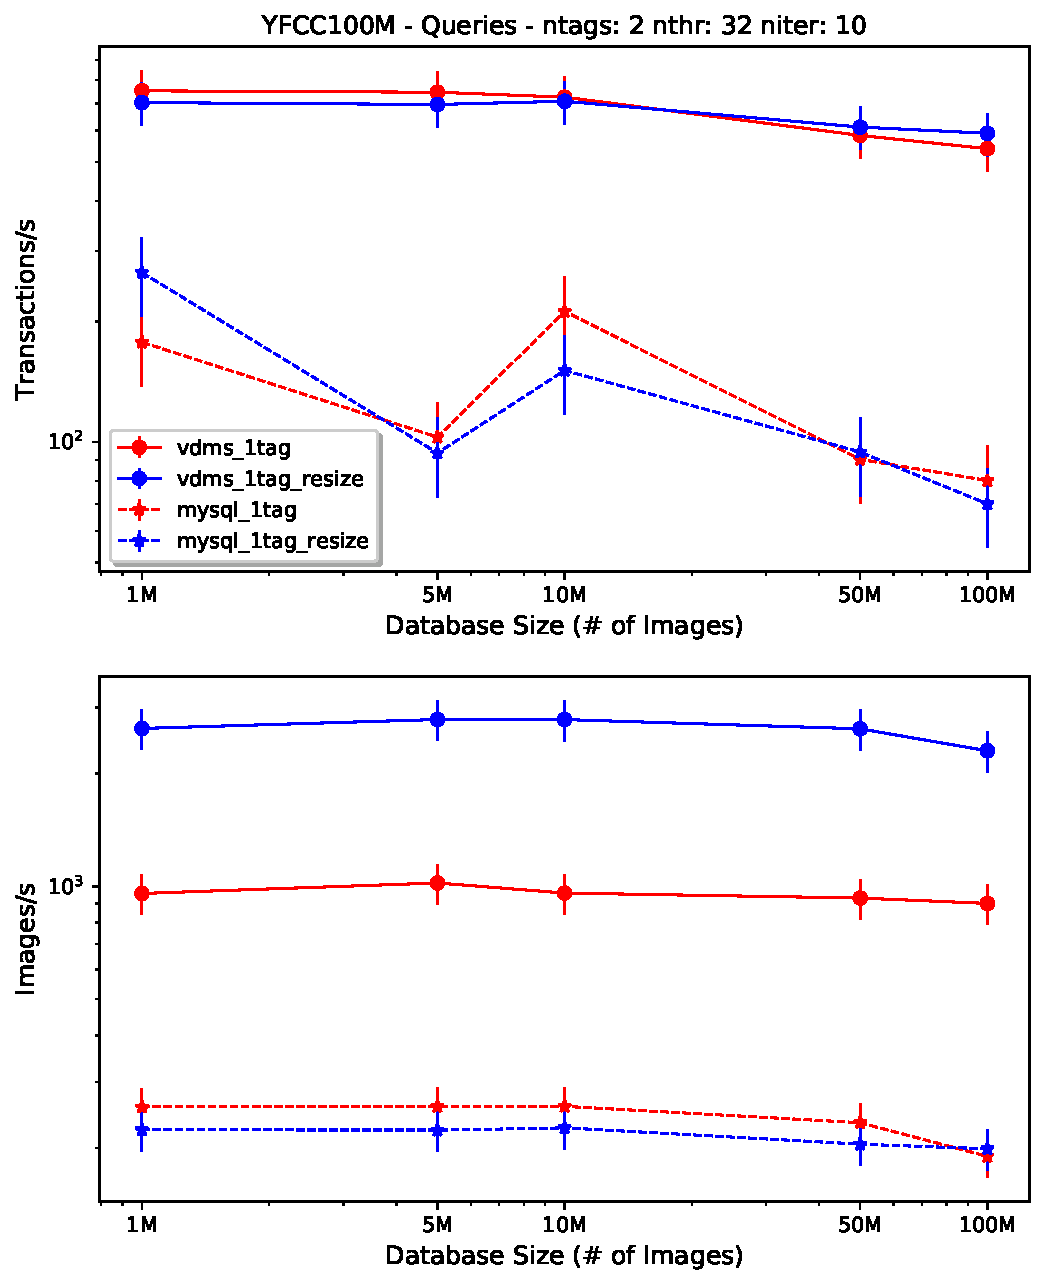
\includegraphics[width=\columnwidth]{figures/queries_throughput_32}
\caption{Queries - Throughput - 32 Clients}
\label{fig:q_throughput_32}
\end{figure}

\begin{figure}[t!]
\centering
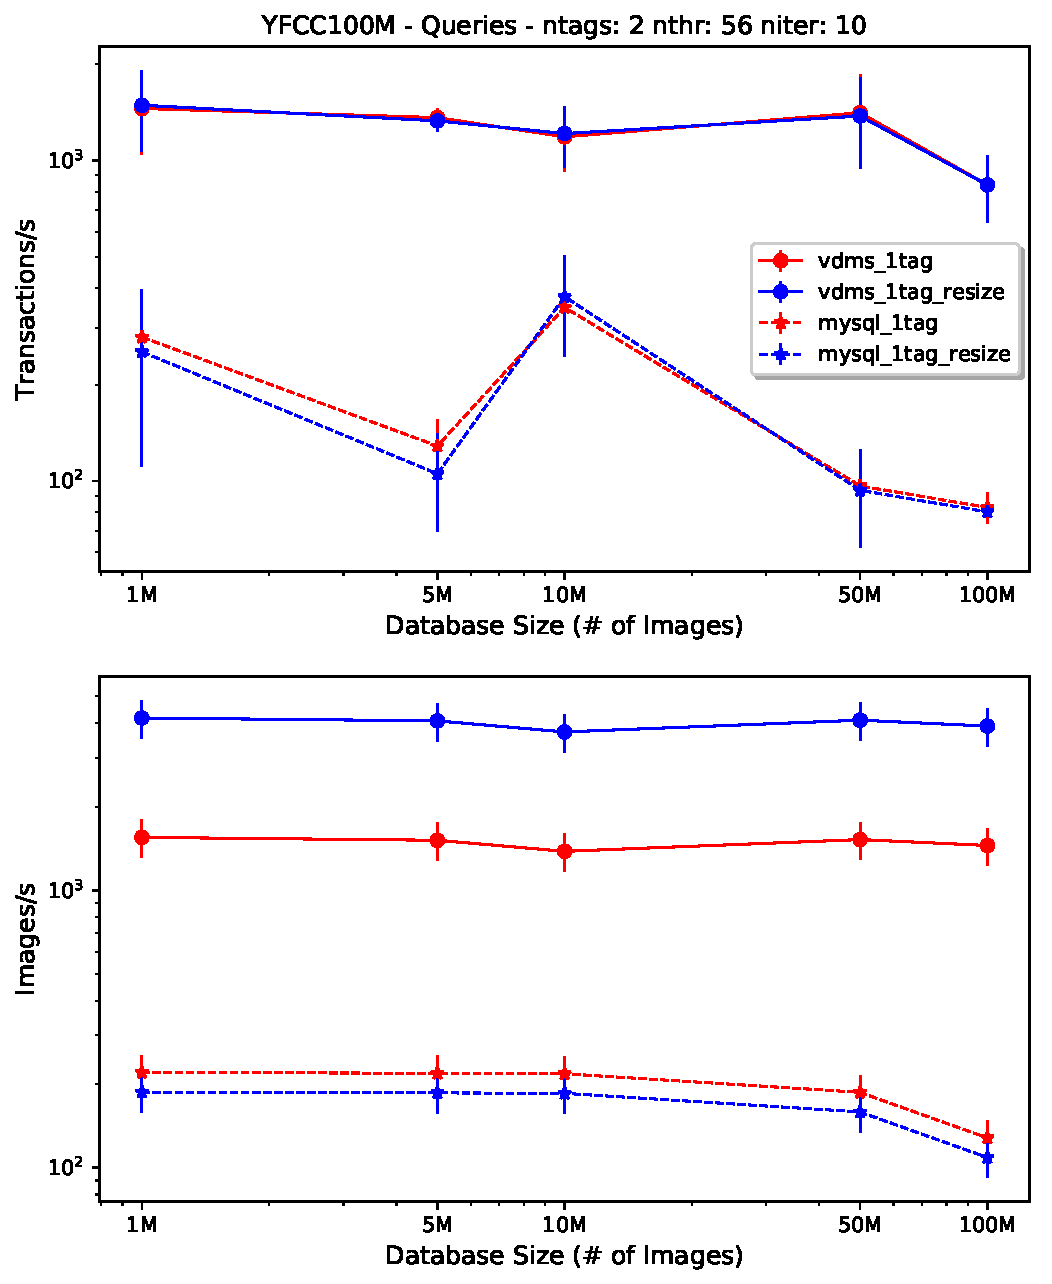
\includegraphics[width=\columnwidth]{figures/queries_throughput_56}
\caption{Queries - Throughput - 56 Clients}
\label{fig:q_throughput_56}
\end{figure}

\subsection{Videos}

\textbf{\textit{Explanation of the video queries and comparison.
Explain concurrency.}}

\begin{figure*}[]
\centering
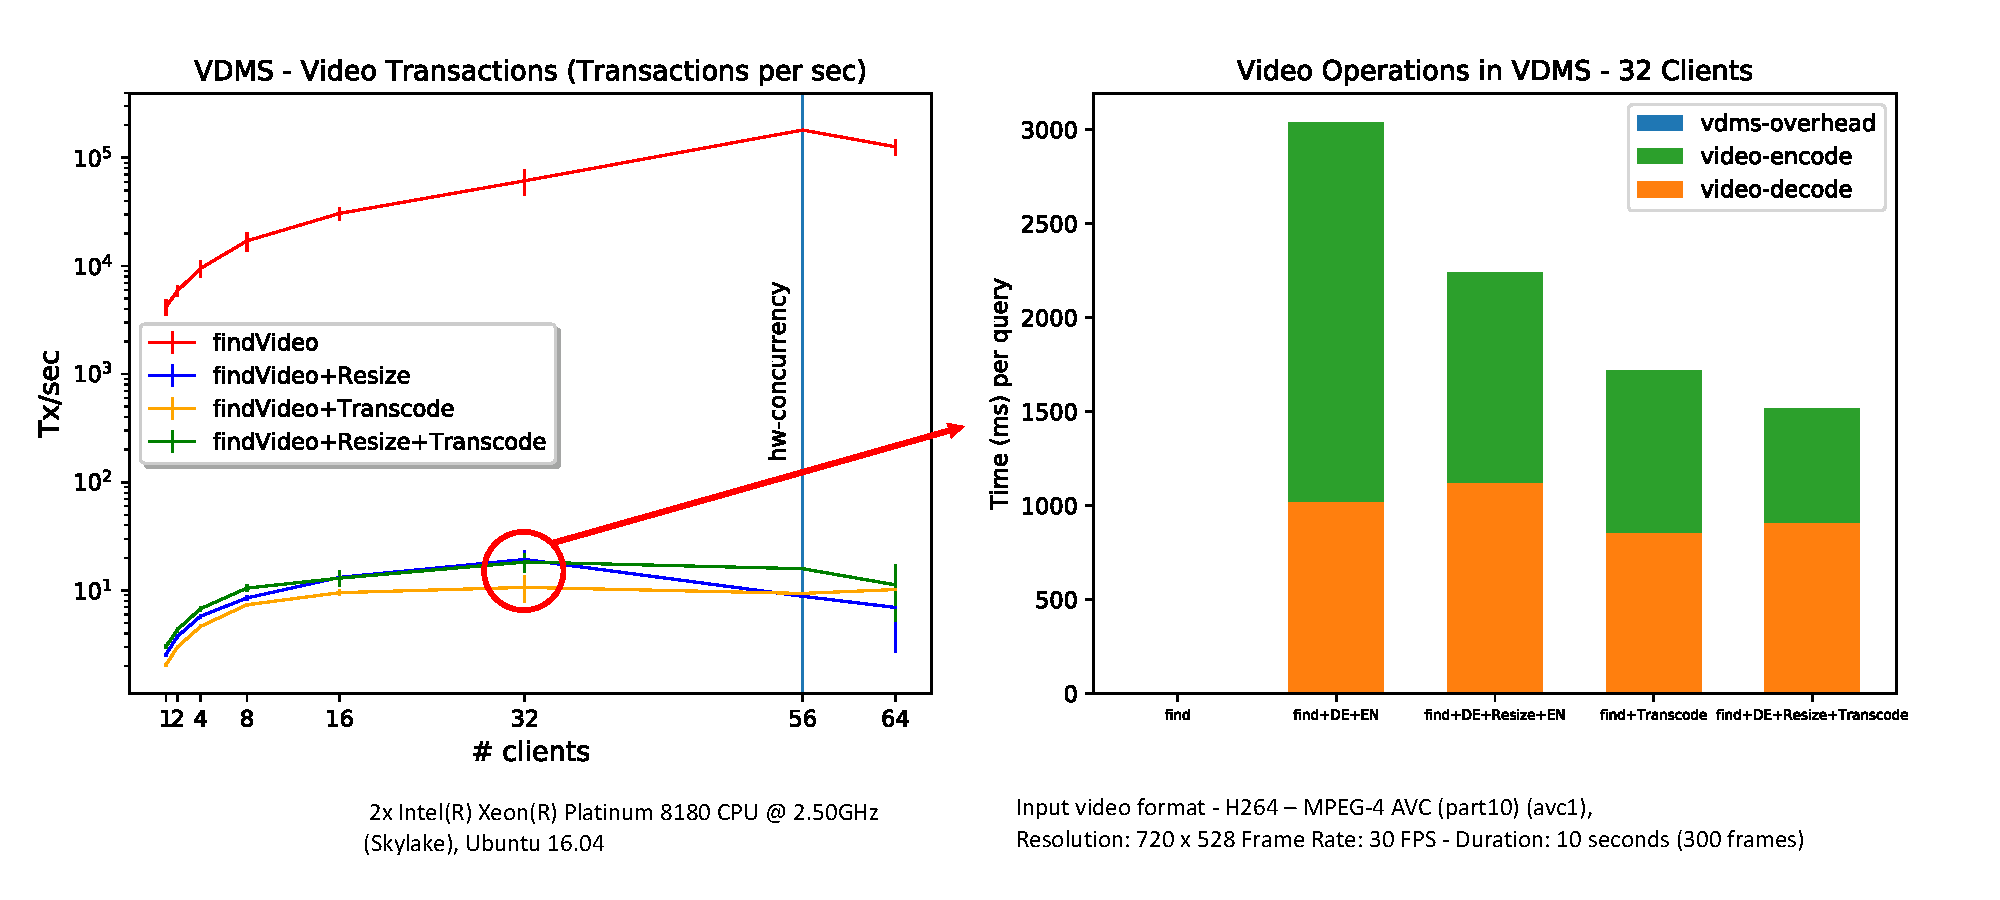
\includegraphics[width=\textwidth]{figures/video_overhead}
\caption{Concurrency and Overhead}
\label{fig:video}
\end{figure*}

\subsection{Feature Vectors}

\textbf{\textit{Explain different engines supported, and how the features vectors
were ingested and handled.}}

\begin{figure*}[]
\centering
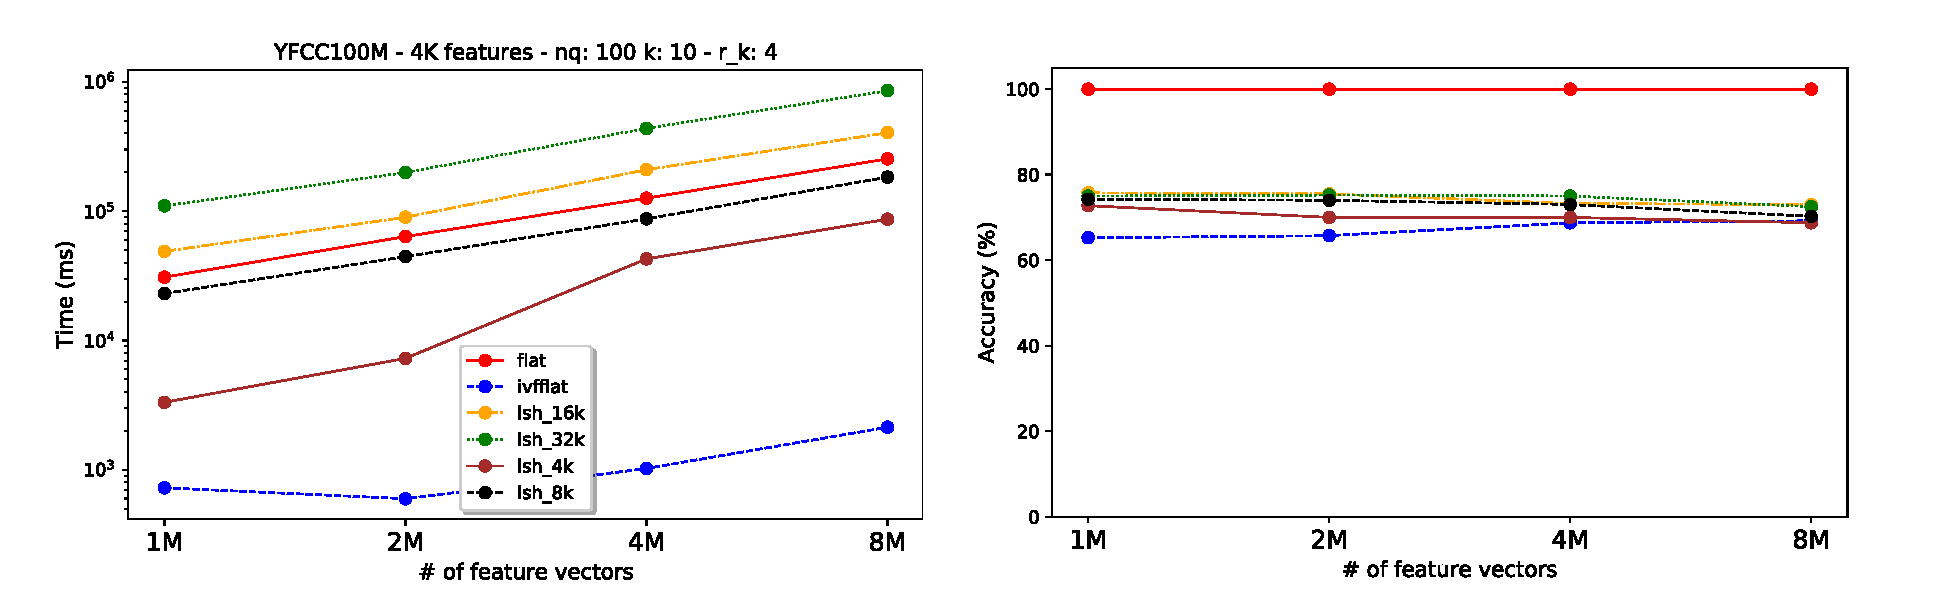
\includegraphics[width=\textwidth]{figures/features_alternatives}
\caption{Feature Vector Evaluation}
\label{fig:features_eval}
\end{figure*}

\begin{figure*}[]
\centering
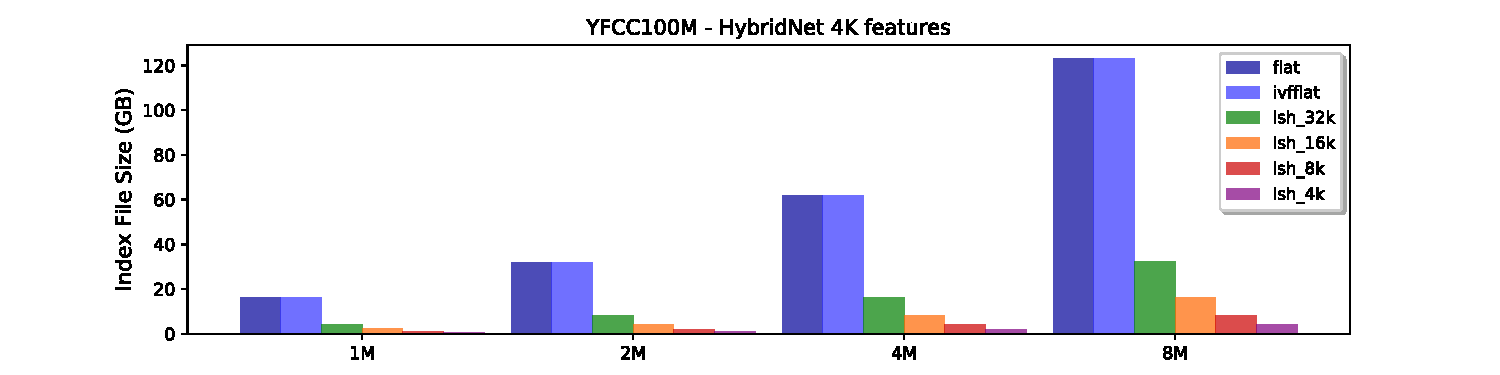
\includegraphics[width=\textwidth]{figures/features_disksize}
\caption{Feature Collection Size in Disk}
\label{fig:features_size_does_matter}
\end{figure*}
